\documentclass{article}
\usepackage[utf8]{inputenc}
\usepackage[margin=1in]{geometry}
\usepackage{tikz}
\usetikzlibrary{graphs,positioning,arrows}


\title{Railroad Diagram}


\begin{document}

\maketitle

\section{MOD BLOCK}
\begin{center}
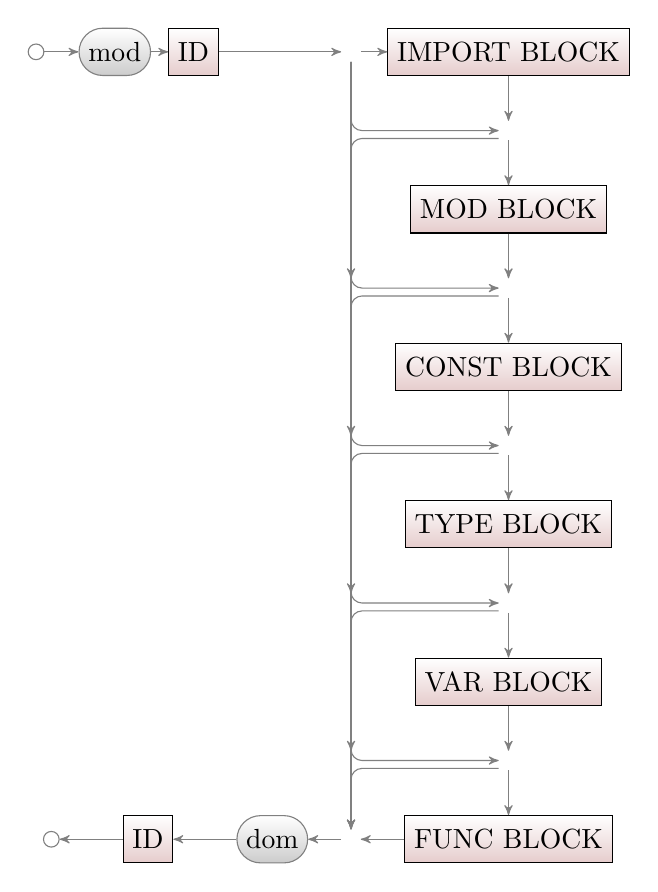
\begin{tikzpicture}[
node distance=8mm,
>=stealth',
black!50,
text=black,
graphs/every graph/.style={edges=rounded corners},
skip loop/.style={to path={-- ++(0,#1) -| (\tikztotarget)}},
hv path/.style={to path={-| (\tikztotarget)}},
vh path/.style={to path={|- (\tikztotarget)}},
box/.style={%
    rectangle,
    minimum size=6mm,
    draw=black,
    top color=white, 
    bottom color=red!50!black!20, 
},
rounded/.style={%
    rectangle,minimum size=6mm,rounded corners=3mm,
    draw=black!50,
    top color=white,bottom color=black!20,
},
start/.style={%
    circle,inner sep=2pt,minimum size=2pt,fill=white,draw=black!50,
},
end/.style={%
    start,
},
]
% Nodes
\node[start]    at (0,0)    (start)             {};
\node[rounded]  at (1, 0)   (mod)               {mod};
\node[box]      at (2, 0)   (modulename)        {ID};
\node           at (4,0)    (nametoimports)     {};

\node[box]      at (6,0)    (imports)           {IMPORT BLOCK};
\node           at (6, -1)  (importstomodules)  {};
\node           at (6, -1.1)(importstorail)     {};

\node[box]      at (6, -2)  (modules)           {MOD BLOCK};
\node           at (6, -3)  (modulestoconsts)   {};
\node           at (6, -3.1)(modulestorail)     {};

\node[box]      at (6, -4)  (constants)         {CONST BLOCK};
\node           at (6, -5)  (conststotypes)     {};
\node           at (6, -5.1)(conststorail)      {};

\node[box]      at (6, -6)  (types)             {TYPE BLOCK};
\node           at (6, -7)  (typestovars)       {};
\node           at (6, -7.1)(typestorail)       {};

\node[box]      at (6, -8)  (variables)         {VAR BLOCK};
\node           at (6, -9)  (varstofuncs)       {};
\node           at (6, -9.1)(varstorail)        {};

\node[box]      at (6, -10) (functions)         {FUNC BLOCK};

\node           at (4, -1)  (modulesempty)      {};
\node           at (4, -3)  (constsempty)       {};
\node           at (4, -5)  (typesempty)        {};
\node           at (4, -7)  (varsempty)         {};
\node           at (4, -9)  (funcsempty)        {};

\node           at (4, -10) (funcstodom)        {};

\node[rounded]  at (3, -10) (dom)              {dom};
\node[box,left=of dom]      (modulenameend)    {ID};
\node[end,left=of modulenameend](end)          {};

% Lines
\graph [use existing nodes] {
    start -> mod -> modulename -> nametoimports -> imports;
    imports -> importstomodules -> modules;
    modules -> modulestoconsts -> constants;
    constants -> conststotypes -> types;
    types -> typestovars -> variables;
    variables -> varstofuncs -> functions;
    functions -> funcstodom;
    funcsempty -> funcstodom;
    funcstodom -> dom;
    dom -> modulenameend;
    modulenameend -> end;
    nametoimports -> funcstodom;
    nametoimports ->[vh path] importstomodules;
    modulesempty ->[vh path] modulestoconsts;
    constsempty ->[vh path] conststotypes;
    typesempty ->[vh path] typestovars;
    varsempty ->[vh path] varstofuncs;
    
    importstorail ->[hv path] constsempty;
    modulestorail ->[hv path] typesempty;
    conststorail ->[hv path] varsempty;
    typestorail ->[hv path] funcsempty;
    varstorail ->[hv path] funcstodom;
};
\end{tikzpicture}
\end{center}
\end{document}
